\documentclass[polish,10pt]{article}
\usepackage[T1]{fontenc}
\usepackage{polski}
\usepackage{amsmath}
\usepackage{graphicx}
\usepackage{pbox}
\usepackage{url}

\title{Elementy kombinatoryki}
\author{Valerija Artiomova \\
	Uniwersytet Gdański}

\date{\today}
\begin{document}
\nocite{*}
\begin{titlepage}
\maketitle

\begin{abstract}
Kombinatoryka jest działem matematyki, który pomaga odpowiedzieć na pytania typu: "ile jest możliwych wyników w rzucie monetą?", "Na ile sposobów możemy wybrać delegację dwuosobową z klasy 28 osobowej?", itp.
Aby rozwiązać tego typu zadania, często stosuje się wzory na permutacje, kombinacje, wariacje oraz wariacje z powtórzeniami.
Na szczęście nie trzeba pamiętać tych wszystkich wzorów, aby szybko i skutecznie rozwiązywać zadania z kombinatoryki.
Do rozwiązania większości zadań w zupełności wystarcza reguła mnożenia i wzór na kombinację.
\end{abstract}
\begin{center}
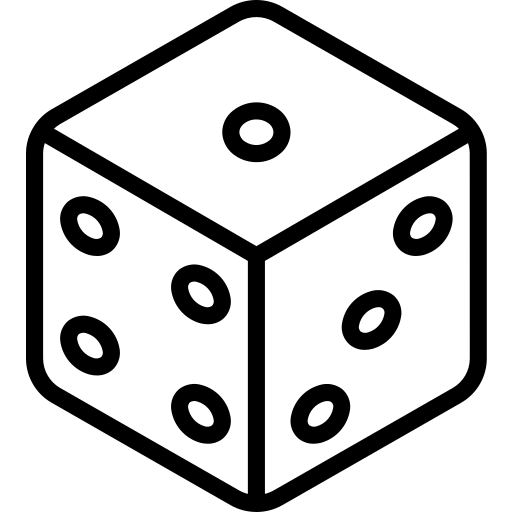
\includegraphics[scale=0.2, ]{images/cube.jpeg}
\end{center}
\end{titlepage}


\section{Reguła mnożenia}
Reguła mnożenia przydaje się podczas rozwiązywania wielu zadań z kombinatoryki.\cite{RM}
\paragraph{Przykład 1.}
\underline{Rzucamy trzy razy monetą.} Ile jest wszystkich możliwych wyników tego doświadczenia?

\hspace{1cm}\\Rozwiązanie: 
Możliwe wyniki to np.: \textbf{(Orzeł,Orzeł,Reszka), (O,R,R), (R,O,R), (R,R,R)...}\cite{WK}
\hspace{1cm}\\Zatem: 

\begin{itemize}
\item W I rzucie może wypaść orzeł lub reszka, czyli są 2 możliwości. 
\item W II rzucie również może wypaść orzeł lub reszka, czyli są 2 możliwości.
\item W III rzucie również może wypaść orzeł lub reszka, czyli są 2 możliwości.
\end{itemize}

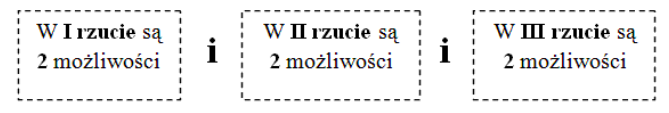
\includegraphics[width=\textwidth]{images/rzuty.png}

\hspace{1cm}\\Reguła mnożenia mówi, że w takiej sytuacji mamy:  
\begin{equation*}
2\cdot2=8
\end{equation*}
możliwości. 

\hspace{1cm}\\
\underline{W regule mnożenia zawsze zamieniamy spójnik $i$ na mnożenie.}

\paragraph{Przykład 2.}
Obliczmy, ile jest wszystkich liczb czterocyfrowych, w których zapisie występują tylko cyfry 3 i 4.

\hspace{1cm}\\Pierwszy element ciągu (cyfrę tysięcy danej liczby) możemy wybrać na dwa sposoby, na drugim miejscu (cyfra setek) też możemy umieścić jedną z dwóch cyfr. Tak więc na dwóch pierwszych miejscach możemy umieścić cyfry na 4 sposoby. Na trzecim (cyfra dziesiątek) i czwartym (cyfra jedności) miejscu możemy również umieścić cyfry 3 lub 4. A więc liczba wszystkich możliwości wynosi
\begin{equation*}
4\cdot2\cdot2\cdot2\cdot2=2^4=16
\end{equation*}
Tłumacząc to zagadnienie na język matematyki, pytamy, ile ciągów czterowyrazowych możemy zbudować ze zbioru dwuelementowego, jeżeli elementy mogą się powtarzać.\cite{ME}
\\Każdy taki czterowyrazowy ciąg utworzony z cyfr 3 i 4, w którym elementy
mogą się powtarzać, nazywamy czterowyrazową wariacją z powtórzeniami
zbioru dwuelementowego $\{3,4\}$.

\noindent\fbox{%
    \parbox{\textwidth}{%
        Wariacją $k$-wyrazową z powtórzeniami zbioru $n$-elementowego, gdzie $k,n \in \mathbb{N_+}$, nazywamy każdy $k$-wyrazowy ciąg utworzony z $k$ niekoniecznie różnych elementów tego zbioru.
    }%
}

\hspace{1cm}\\Jeżeli ze zbioru składającego się z $n$ elementów wybieramy $k$ elementów $(k \leq n)$, w ten sposób, że:

\begin{itemize}
\item istotna jest kolejność wybieranych elementów
\item wybierane elementy mogą się powtarzać, to w ten sposób budujemy k-wyrazową wariację z powtórzeniami tego zbioru.
\end{itemize}
\paragraph{Ćwiczenie 1.}
Ile jest wszystkich liczb czterocyfrowych, w których zapisie mogą występować tylko cyfry 1, 2 i 3?
\paragraph{Przykład 3.}
Dany jest zbiór Z składający się z liczb 5, 6, 7, 8, 9, 
czyli $Z=\{5, 6, 7, 8, 9\}$.

\hspace{1cm}\\Ponieważ możemy utworzyć pięć jednowyrazowych ciągów z elementów zbioru Z, więc
mamy pięć jednowyrazowych wariacji z powtórzeniami. Są nimi jednowyrazowe ciągi (5), (6), (7), (8), (9). Zatem $W^1_5 = 5$.

\hspace{1cm}\\Dopisując w powyższych wariacjach na drugim miejscu kolejno elementy zbioru Z, otrzymamy dwuwyrazowe wariacje z powtórzeniami zbioru Z:

\hspace{1cm}\\(5,5), (5,6), (5,7), (5,8), (5,9),
\\(6,5), (6,6), (6,7), (6,8), (6,9),
\\(7,5), (7,6), (7,7), (7,8), (7,9),
\\(8,5), (8,6), (8,7), (8,8), (8,9),
\\(9,5), (9,6), (9,7), (9,8), (9,9).

\hspace{1cm}\\Zatem $W^2_5=5\cdotW^1_5=5\cdot5=5^2$.

\hspace{1cm}\\Dalej weźmy dwuwyrazowe wariacje z powtórzeniami zaczynające się od liczby 5 i dopiszmy na trzecim miejscu kolejno elementy zbioru Z, otrzymując trzyelementowe wariacje zbioru Z:

\hspace{1cm}\\(5,5,5), (5,5,6), (5,5,7), (5,5,8), (5,5,9),
\\(5,6,5), (5,6,6), (5,6,7), (5,6,8), (5,6,9),
\\(5,7,5), (5,7,6), (5,7,7), (5,7,8), (5,7,9),
\\(5,8,5), (5,8,6), (5,8,7), (5,8,8), (5,8,9),
\\(5,9,5), (5,9,6), (5,9,7), (5,9,8), (5,9,9).


\hspace{1cm}\\Postępując analogicznie z pozostałymi dwuwyrazowymi wariacjami, dochodzimy do wniosku, że  $W^3_5 = 5\cdot W^2_5 = 5\cdotW^1_5 = 5\cdot5=5^3$.
\hspace{1cm}\\Następnie, biorąc trzywyrazowe wariacje z powtórzeniami i dopisując na czwartym miejscu kolejno elementy zbioru Z, otrzymujemy czteroelementowe wariacje z powtórzeniami zbioru Z.
Rozumując tak jak wyżej, mamy $W^4_5 = 5\cdot W^3_5 = 5\cdot W^2_5 = 5\cdotW^1_5 = 5\cdot5=5^4$.



\hspace{1cm}\\\noindent\fbox{%
    \parbox{\textwidth}{%
        Liczba wszystkich $k$-wyrazowych wariacji z powtórzeniami zbioru $n$ elementowego wyraża się wzorem $W^k_n=n^k$.
    }%
}
\paragraph{Przykład 4.}
Obliczmy, ile jest wszystkich liczb dwucyfrowych, w których zapisie występują tylko cyfry 1, 2, 3, 4, 5 i żadna z cyfr się nie powtarza.

\hspace{1cm}\\Zauważmy, że pierwszą cyfrę możemy wybrać na 5 sposobów, a drugą na 4 sposoby. Zgodnie z regułą mnożenia otrzymujemy $5\cdot4=20$ . Są to następujące liczby:

\hspace{1cm}\\12, 13, 14, 15, 21, 23, 24, 25, 31, 32, 34, 35, 41, 42, 43, 45, 51, 52, 53, 54.

\hspace{1cm}\\Stosując język matematyki, pytamy, ile ciągów dwuwyrazowych możemy zbudować, używając różnych elementów zbioru $\{1, 2, 3, 4, 5\}$.

\hspace{1cm}\\Każdy taki dwuwyrazowy ciąg utworzony z cyfr 1, 2, 3, 4, 5, w którym wyrazy nie powtarzają się, nazywamy dwuwyrazową wariacją bez powtórzeń zbioru {1, 2, 3, 4, 5}.

\hspace{1cm}\\\noindent\fbox{%
    \parbox{\textwidth}{%
        Wariacją $k$-wyrazową bez powtórzeń zbioru $n$-elementowego, gdzie $k,n \in \mathbb{N_+}$, oraz $k \leq n$, nazywamy każdy k-wyrazowy ciąg utworzony z $k$ różnych elementów tego zbioru.
    }%
}
\paragraph{Ćwiczenie 2.}
Ile jest wszystkich liczb pięciocyfrowych, w których zapisie mogą występować tylko cyfry 1, 2, 3, 4, 5, 6, 7, 8, 9 i żadna cyfra się nie powtarza?

\paragraph{Przykład 4.}
Dany jest zbiór Z składający się z liczb 5, 6, 7, 8, 9, czyli $Z =\{5, 6, 7, 8, 9\}$.

\hspace{1cm}\\Mamy pięć jednowyrazowych wariacji bez powtórzeń, są nimi jednowyrazowe ciągi

\hspace{1cm}\\(5), (6), (7), (8), (9),

\hspace{1cm}\\więc $V^1_5 = 5$.

\hspace{1cm}\\Dopisując w powyższych wariacjach na drugim miejscu kolejno elementy zbioru Z niewystępujące w tej wariacji, otrzymamy dwuwyrazowe wariacje bez powtórzeń zbioru Z:

\hspace{1cm}\\(5,5), (5,6), (5,7), (5,8), (5,9),
\\(6,5), (6,6), (6,7), (6,8), (6,9),
\\(7,5), (7,6), (7,7), (7,8), (7,9),
\\(8,5), (8,6), (8,7), (8,8), (8,9),
\\(9,5), (9,6), (9,7), (9,8), (9,9).

\hspace{1cm}\\ więc $V^2_5 = 4 \cdot V^1_5 = 4\cdot5$.

\hspace{1cm}\\Dalej weźmy dwuwyrazowe wariacje bez powtórzeń i dopiszmy na trzecim miejscu kolejno elementy zbioru Z niewystępujące w tej wariacji. Otrzymamy trzyelementowe wariacje bez powtórzeń zbioru Z.

\hspace{1cm}\\(5,6,7), (5,6,8), (5,6,9),
\\(5,7,6), (5,7,8), (5,7,9), 
\\(5,8,6), (5,8,7), (5,8,9), 
\\(5,9,6), (5,9,7), (5,9,8). 


\hspace{1cm}\\Postępując analogicznie z pozostałymi dwuwyrazowymi wariacjami, dochodzimy do wniosku, że $V^3_5 = 3 \cdot V^2_5 = 3\cdot4\cdot5$.

\hspace{1cm}\\Następnie do trzywyrazowych wariacji z powtórzeniami dopiszemy na czwartym miejscu kolejno elementy zbioru $Z$. Otrzymamy czteroelementowe wariacje bez powtórzeń zbioru $Z$.

\hspace{1cm}\\W wyniku otrzymujemy $V^4_5 = 2\cdot V^3_5 = 3\cdot4\cdot5$.

\hspace{1cm}\\\noindent\fbox{%
    \parbox{\textwidth}{%
        Liczba wszystkich $k$-wyrazowych wariacji bez powtórzeń zbioru $n$-elementowego,gdzie $k,n \in \mathbb{N_+}$ oraz $k \leq n$ , wyraża się wzorem $V^k_n = n(n-1)(n-2)\dots(n-k+1)$.
    }%
}

\hspace{1cm}\\Twierdzenie można udowodnić za pomocą indukcji matematycznej.

\section{Bibliografia}
\bibliographystyle{plain}
\bibliography{data.bib}

\end{document}